\documentclass[a4paper,11pt, twoside]{article}
\usepackage{graphicx,listings,float,geometry, amsmath,placeins}
%\usepackage[firstpage]{draftwatermark}
%\SetWatermarkLightness{0.5}
%\SetWatermarkScale{4}
\setcounter{tocdepth}{2}
\usepackage[dutch]{babel}
\usepackage{xspace, color,mdframed}
\usepackage[usenames,dvipsnames]{xcolor}

\geometry{
	includeheadfoot,
	margin=2.54cm
}
\newcommand{\BS}{BrnStrm}
\newcommand{\ON}{Ori\"entatie}
\newcommand{\MW}{Werkplan}
\newcommand{\MS}{SpelSpec}
\newcommand{\MA}{Spelkeus}
\newcommand{\BO}{Deel. Docu.}
\newcommand{\OC}{Protocol}
\newcommand{\MN}{Impl.Proto.}
\newcommand{\CT}{Proto Test}
\newcommand{\MK}{Klas.diagr.}
\newcommand{\MT}{Taakverdel.}
\newcommand{\IS}{Implement}
\newcommand{\BG}{Handl.}
\newcommand{\AV}{Eind Docu}
\newcommand{\ME}{Mkn.prsnt.}
\newcommand{\EP}{Presenteren}

\begin{document}
	\begin{titlepage}
	\begin{center}
		
		{\Huge Informele Specificatie \\[0.5cm]OGO 2.3 - Multiplayer Game}\\[0.5cm]
		\rule{\linewidth}{0.5mm}\\[0.5cm]
				\bigskip
		\huge \textit{``Grudge of the Oblivious''}
		
		{\Large
		Luca van Ballegooijen, Tim van Dalen, \\
		Carl van Dueren den Hollander, Peter Koymans,\\
		Kay Lukas en Ferry Timmers\\[1cm]
		}
		
		{\large
		OGO 2.3\\
		Groep 3 \\[1cm]
		Faculteit Wiskunde en Informatica\\
		Technische Universiteit Eindhoven\\[1cm]
		}
		
		\begin{abstract}

    In dit document zullen we de kritieke punten bij dit project identificeren. Vervolgens bekijken we de taken die bij dit project een rol spelen. Tenslotte zullen we dit gebruiken om een werkplan voor het project op te stellen.
\end{abstract}


		\vfill

		{\large \today}
	\end{center}
\end{titlepage}

    % Mist nog:
    % - Nummer vak (2IO46)
    % - Identiteitsnummers groepsleden
    % -	Naam tutor (Mels van Broekhoven)

	\tableofcontents
	\newpage

	\section{Lijst symbolen en afkortingen}
    % Verklaring van alle gebruikte symbolen	

    \section{Summary}
    % Engelstalige samenvatting

    \section{Inleiding}
    Informatici in de hedendaagse wereld komen vaak in aanraking met het ontwerpen van complexe programma's. Complexe programma's hebben vaak ook een netwerk aspect en een grafische aspect. Zelfs bij technische programma's, die vaak minder grafisch intensief zijn, als matlab worden al deze aspecten verenigd. Dit drukt de noodzaak uit dat elke informaticus basiskennis heeft van computergrafiek, computernetwerken en het ontwerpen van complexe programma's. Al deze aspecten worden verenigd in dit project: \textsc{ogo} 2.3 - Nethunt. Dit document ligt ... INSERT MORE

Voor dit project werd ons gevraagd om een interactief, gedistribueerd 3D-spel te ontwikkelen. Dit houdt in dat elk speler lokaal dezelfde spelsituatie heeft, en deze op het scherm van de speler worden afgebeeld. Natuurlijk kan de afbeelding op het scherm verschillen per speler. Een andere eis was dat er voedsel aanwezig moet zijn. E\'en van de randvoorwaarden was dat elke speler ... INSERT MORE
    % Probleem- of vraagstelling
    % Opbouw

    \section{Hoofdtekst}
    % Waarschijnlijk beter aparte sections

    \subsection{Werkplan}
    % Intro werkplan.
    INSERT INTRO WERKPLAN.
    
    \subsubsection{Kritieke punten}
    We identificeren eerst de kritieke punten in dit project, voordat we het werkplan geven. Dit zijn:
    \begin{enumerate}
    \item[(a)] Het eerste kritieke punt is het netwerk aspect. Ten eerste moet het mogelijk zijn om elkaar te kunnen vinden over het netwerk. Dit is zeker geen triviale taak. Ten tweede geldt dat gedurende het spel alle machines op gelijke voet staan. Er mag dus geen server worden gebruikt, wat het ontwerp van het spel moeilijker maakt.
    \item[(b)] Een ander groot gevaar is complexiteit. Bij het ontwikkelen van een spel kan men al snel uit enthousiasme hoge verwachtingen krijgen en hoge eisen stellen. Deze overmaat aan eisen kan later te veel werk blijken.
    \item[(c)] Een laatste hindernis is het gedistribueerde aspect met name in conflictsituaties. Een goed voorbeeld hiervan is als twee spelers op hetzelfde moment voedsel proberen te pakken. 
    \end{enumerate}
    
    We willen zo vroeg mogelijk aan deze kritieke punten werken. Aangezien we (a) als het voornaamste probleem beschouwen, zullen we in week 1 ons al ori\"enteren op het probleem. We zullen vooral kijken naar de mogelijkheden voor broadcast om andere spelers te vinden.
    
    \subsubsection{De taken}
    Nu we de mogelijke problemen hebben bekeken, zijn we klaar om een lijst met taken op te stellen met afkortingen. De genoemde taken staan ruwweg in chronologische volgorde:
    \begin{enumerate}
    \item[-] Brainstormen over spelidee (\emph{\BS}).
    \item[-] Ori\"entatie op netwerk aspect door het maken van eenvoudig chat programma (\emph{\ON}).
    \item[-] Maken werkplan met taakverdeling (\emph{\MW}).
    \item[-] Maken spelspecificatie en gebruikershandleiding (\emph{\MS}).
    \item[-] Maken alternatieven en motivering van spelkeuze (\emph{\MA}).
    \item[-] Beschrijving onderdelen en onderlinge samenhang (\emph{\BO}).
    \item[-] Ontwerpen communicatieprotocol (\emph{\OC}).
    \item[-] Maken onderliggende netwerkcommunicatie (\emph{\MN}).
    \item[-] Communicatieprotocol testen (\emph{\CT}).
    \item[-] Maken klassendiagram (\emph{\MK}).
    \item[-] Maken taakverdeling voor implementatie (\emph{\MT}).
    \item[-] Maken modellen en textures, inladen in openGL (\emph{Model}).
    \item[-] Maken basisklassen (\emph{Basis}).
    \item[-] Maken lobby (\emph{Lobby}).
    \item[-] Maken gebruikersomgeving (\emph{Gbr}).    
    \item[-] Bijwerken gebruikershandleiding, validatie aannames en motivering implementatie (\emph{\BG}).
    \item[-] Afronden verslag (\emph{\AV}).
    \item[-] Maken eindpresentatie (\emph{\ME}).
    \item[-] Eindpresentatie (\emph{\EP}).
    \end{enumerate}

    \subsubsection{Het werkplan}
    Als laatste moeten de taken nog over de personen worden verdeeld. Hierbij zullen we taken proberen te rouleren zodanig dat iedereen zowel taken heeft voor programmeren als documenteren. Aangezien wij allemaal zowel ervaring hebben met programmeren als met documenteren, zullen we bij de taakverdeling geen speciale rekening houden met de koppels (bijvoorbeeld relatief goede programmeurs bij relatief zwakke programmeurs). 
    
    Het is daarbij belangrijk om in te zien dat de genoemde taken redelijk onafhankelijk van elkaar zijn uit te voeren. We proberen er in de taakverdeling voor te zorgen dat een klein aantal groepen zo onafhankelijk mogelijk van de rest kan werken. Om dit te bereiken, werken we zoveel mogelijk \emph{bottom-up}. Verder hebben we als doel dat iedereen met de verschillende aspecten van het programma te maken krijgt. Het protocol is al gezamenlijk ontworpen en getest, zodat iedereen met het gedistribueerde aspect te maken heeft gehad. We zullen met deze taakverdeling proberen iedereen ook te laten werken aan het grafische aspect.

    We hebben besloten om drie belangrijke zaken samen te doen. Ten eerste is het natuurlijk erg logisch dat het brainstormen samen gebeurt. Hierdoor weten we allemaal in welke richting het spel zal gaan, wat bij alle volgende stappen van belang zal zijn. Ten tweede wordt het communicatieprotocol samen ontworpen. Dit heeft tot doel zodat iedereen het communicatieprotocol goed snapt, zodat iedereen hiermee overweg kan met de implementatie. Ten derde wordt het testen van het communicatieprotocol samen gedaan. De voornaamste reden hiervoor is vanwege de grote diversiteit aan operating systemen in onze groep, wat eventueel problemen kan geven bij de implementatie. We zijn nu klaar om het volledige werkplan te geven, we gebruiken hierbij de eerder gegeven afkortingen. De deadlines staan op een aparte regel en zijn schuin gedrukt:
    \begin{figure}[H]
        \small
        \centering
        \begin{tabular}{| l | l | l | l | l | l | l |}
        \hline
        Week & Carl & Ferry & Kay & Luca & Peter & Tim \\ \hline
        Week 1 24-04-2012 & \BS & \BS & \BS & \BS & \BS & \BS \\ \hline
        Week 1 25-04-2012 & \ON & \ON & \ON & \ON & \MW & \ON \\ \hline
        Week 1 26-04-2012 & \ON & \ON & \ON & \ON & \MW & \ON \\ \hline
        Week 2 01-05-2012 & \MS & \MA & \MA & \MS & \MA & \MS \\ \hline
        Week 2 02-05-2012 & \MS & \MA & \MA & \MS & \MA & \MS \\ \hline
        Week 2 03-05-2012 & \MS & \MA & \MA & \MS & \MA & \MS \\ \hline
        Week 2 04-05-2012 & \multicolumn{6}{|c|}{\emph{Deadline ori\"entatiefase}} \\ \hline
        Week 3 08-05-2012 & \MS & \MA & \MA & \MS & \MA & \MS \\ \hline
        Week 3 09-05-2012 & \MS & \MA & \MA & \MS & \MA & \MS \\ \hline
        Week 3 10-05-2012 & \MS & \MA & \MA & \MS & \MA & \MS \\ \hline
        Week 4 15-05-2012 & \OC & \OC & \OC & \OC & \OC & \OC \\ \hline
        Week 4 16-05-2012 & \OC & \OC & \OC & \OC & \OC & \OC \\ \hline
        Week 4 16-05-2012 & \multicolumn{6}{|c|}{\emph{Deadline specificatiefase}} \\ \hline
        Week 5 22-05-2012 & \BO & \MN & \MK & \MK & \BO & \MN \\ \hline
        Week 5 23-05-2012 & \BO & \MN & \MK & \MK & \BO & \MN \\ \hline
        Week 5 24-05-2012 & \BO & \MN & \MK & \MT & \BO & \MN \\ \hline
        Week 6 30-05-2012 & \BO & \MN & \MK & \MT & \BO & \MN \\ \hline
        Week 6 31-05-2012 & \CT & \CT & \CT & \CT & \CT & \CT \\ \hline
        Week 6 01-06-2012 & \multicolumn{6}{|c|}{\emph{Deadline ontwerpfase}} \\ \hline
        Week 7 05-06-2012 & Model & Basis & Lobby & Basis & Basis & Lobby \\ \hline
        Week 7 06-06-2012 & Model & Basis & Lobby & Basis & Basis & Lobby \\ \hline
        Week 7 07-06-2012 & Model & Basis & Lobby & Basis & Basis & Lobby \\ \hline
        Week 8 12-06-2012 & \BG & Sc\`ene & Sc\`ene & Gbr & Gbr & \BG \\ \hline
        Week 8 13-06-2012 & \BG & Sc\`ene & Sc\`ene & Gbr & Gbr & \BG \\ \hline
        Week 8 14-06-2012 & \BG & Sc\`ene & Sc\`ene & Gbr & Gbr & \BG \\ \hline
        Week 8 14-06-2012 & \multicolumn{6}{|c|}{\emph{Deadline implementatiefase eerste versie}} \\ \hline
        Week 9 19-06-2012 & \AV & \AV & \ME & \AV & \AV & \ME \\ \hline
        Week 9 20-06-2012 & \AV & \AV & \ME & \AV & \AV & \ME \\ \hline
        Week 9 21-06-2012 & \EP & \EP & \EP & \EP & \EP & \EP \\ \hline
        Week 9 22-06-2012 & \multicolumn{6}{|c|}{\emph{Deadline verslag}} \\ \hline
        \end{tabular}
        \caption{Gedetailleerde taakverdeling per dag}
        \label{tab:planning}
    \end{figure}

    Zoals in de tabel is te zien, zijn er ongeveer twee weken om aan de implementatie te werken. Het idee is dat dan een groot deel van het netwerk aspect, wat het grootste risico heeft om uit te lopen, daarvoor al af te hebben om dit op te vangen. Bij de implementatie moet dus vooral aandacht worden besteed aan het modelleren van de sc`ene en het maken van het spel. Het modelleren van de sc`ene is vrij onafhankelijk van de andere activiteiten. Dit kan worden gebruikt door hier eventueel al eerder mee te beginnen, zeker als we in een van de eerdere fasen tijd over hebben. We hebben besloten het protocol al eerder te maken om onverwachte vertragingen vanwege \emph{bugs} op te kunnen vangen, die in onze mening het meest waarschijnlijk zijn bij dit onderdeel van het programma.
    
    \subsection{Specificaties}
    % Intro specificatie.
    INSERT INTRO SPECIFICATIE.

	\subsubsection{Terrein}
    Het terrein kan in wezen allerlei vormen hebben, voorwaarde hierbij is dat het een eerlijk terrein is voor beide teams. Een team mag dus geen voordeel hebben dankzij de kaart. Een mogelijke manier om dit te bereiken is door de kaart symmetrisch te maken. We eisen bovendien dat de kaart rechthoekig is.

    Op het terrein zijn twee commandocentra geplaatst, voor beide teams een commandocentrum. Het kan gewenst zijn dat elk team bij de start van het spel ook al een aantal extra torens heeft ter bescherming van het commandocentrum. Over het terrein zijn een aantal delfplaatsen verdeeld. Deze zijn eerlijk verdeeld over de kaart. Andere obstakels mogen aanwezig zijn, maar zijn niet noodzakelijkerwijs aanwezig. Alle objecten met uitzondering van spelers worden geplaatst op een rooster. In figuur \ref{fig:map1} en \ref{fig:map2} zijn twee mogelijke beginconfiguraties van het spel getoond.
    \begin{figure}[h]
    \begin{subfigure}{0.5\textwidth}
    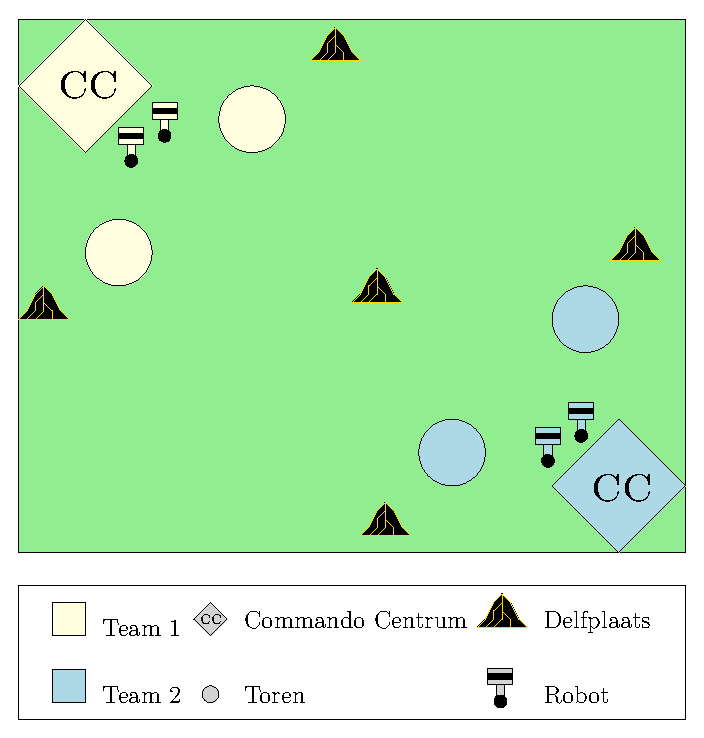
\includegraphics[width=\textwidth]{Graphics/Map1.eps}
    \caption{Een bijna vierkant terrein met vier spelers}
    \label{fig:map1}
    \end{subfigure}\hspace{10mm}
    \begin{subfigure}{0.5\textwidth}
    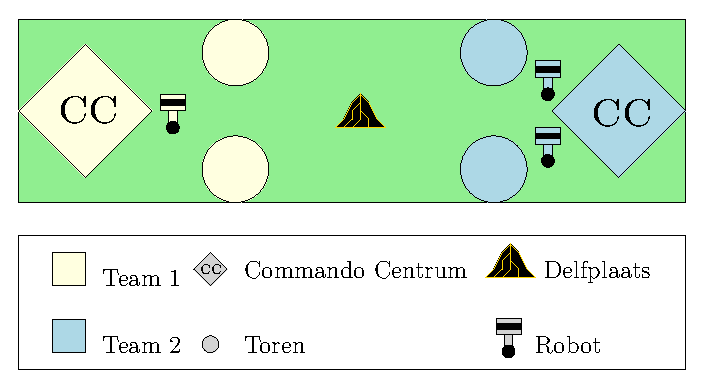
\includegraphics[width=\textwidth]{Graphics/Map2.eps}
    \caption{Een breed terrein met drie spelers}
    \label{fig:map2}
    \end{subfigure}
    \caption{Twee verschillende beginconfiguraties van het spel}
    \end{figure}

    \subsubsection{Spelers}
    Een speler behoort tot \'e\'en van beide teams, spelers van een bepaald team zijn te identificeren door kleuren. De speler ziet de wereld vanuit de positie van zijn robot. Men kan de kijkrichting aanpassen, zodat deze elke willekeurige richting kan zijn. Als de kijkrichting verder naar links of rechts wordt gedraaid, draait de robot mee. De speler heeft een lasergeweer waarmee hij op andere spelers en torens kan schieten om deze te vernietigen. Het lasergeweer schiet laserstralen met een `oneindige' snelheid in de huidige kijkrichting. Dit wordt verder gespecificeerd in de sectie \ref{sec:UI}: \emph{Gebruikersomgeving}. Bij het begin van het spel heeft de robot nog een volledig harnas. Zodra de speler wordt geraakt, wordt de conditie van het harnas slechter. Het is echter niet mogelijk dat een speler het harnas van een andere speler uit hetzelfde team beschadigt.
    \FloatBarrier
    Een speler gaat dood als zijn harnas kapot is. In dat geval zal hij na een bepaalde hoeveelheid tijd terugkeren bij het commandocentrum met een volledig harnas. De conditie van het harnas kan op geen enkele andere dan de hierboven beschreven manieren veranderen. Ook kan een speler gebouwen bouwen, hiervoor gebruikt hij goud uit de kas van het team. De spelers kunnen op het grondvlak bewegen met een vaste snelheid in elke richting. De enige voorwaarde hierbij is dat de spelers op de kaart blijven en niet door een gebouw lopen. Het is dus wel mogelijk dat spelers door elkaar heen kunnen lopen. De speler kijkt vanuit een derde persoon perspectief. In een derde persoon perspectief wordt de sc\`ene bekeken vanaf een punt vlak achter de speler. Het is eventueel mogelijk om dit verder uit te breiden, zodat de speler kan wisselen van derde persoon perspectief naar eerste persoon perspectief.

    \subsubsection{Gebouwen}
    Er zijn drie soorten gebouwen: torens, mijnen en commandocentra. Torens schieten op spelers en andere gebouwen in hun bereik. Mijnen kunnen over delfplaatsen worden gebouwd met het doel de inkomsten van een team te vergroten. In principe levert elke mijn een vaste hoeveelheid goud voor de gezamenlijke kas op. Deze hoeveelheid wordt periodiek toegevoegd aan de kas.

    Uit sommige delfplaatsen kan maar een bepaalde hoeveelheid goud worden gehaald, daarna is de delfplaats op. Dan zal de mijn over die delfplaats geen verdere bijdrage meer leveren voor de gezamenlijke kas. We staan echter ook delfplaatsen toe die een onbeperkte hoeveelheid goud bevatten. Standaard levert elke mijn hetzelfde bedrag op met dezelfde periode, maar dit kan later nog worden aangepast.

    Het commandocentrum is het belangrijkste gebouw voor het team. Als dit gebouw kapot is, heeft het bijbehorende team verloren. Gebouwen kunnen door spelers worden beschoten, waardoor deze worden beschadigd. Gebouwen kunnen op geen enkele mogelijke manier hersteld worden. Optioneel zou men mechanismen in het spel kunnen toevoegen om deze gebouwen te herstellen. Alle gebouwen behoren tot \'e\'en van beide teams, deze gebouwen kunnen weer ge\"identificeerd worden door de kleur van het gebouw.

    \subsubsection{Verzamelbare voorwerpen}
    Er is maar \'e\'en verzamelbaar voorwerp: een muntje. E\'en of meerdere muntjes worden achtergelaten door spelers die dood gaan en torens die worden vernietigd. Een muntje heeft een bepaalde waarde in goud. De waarde van de muntjes zijn proportioneel aan de gezamenlijke kas van het team waarvan de speler is doodgegaan. Als een toren is vernietigd, dan is de waarde van de muntjes proportioneel aan de kosten van de toren. De waarde van de muntjes moet echter altijd kleiner zijn dan de kosten van de toren. Gedurende een spel moeten deze proporties vast zijn.

    Als een speler doodgaat, wordt bovendien nog de waarde van de muntjes afgetrokken van de gezamenlijke kas van die speler. Een muntje kan vervolgens opgepakt worden door alle spelers. Het muntje is dus het voedsel element in ons spel. De waarde van het muntje zal dan toegevoegd worden aan de kas van het bijbehorende team.

    \subsubsection{Initialisatie}
    De spelers kunnen zelf kiezen bij welk team ze gaan, onder de voorwaarde dat elk team minstens \'e\'en speler heeft. Bij de start van het spel staan alle spelers bij het commandocentrum. Zoals al eerder gezegd, hebben alle spelers dan nog een volledig harnas. Bovendien heeft elk team een zekere positieve hoeveelheid goud in de gezamenlijke kas, die voor beide teams natuurlijk gelijk moet zijn. Er kunnen minstens twee mijnen gebouwd worden met deze hoeveelheid goud.
    \FloatBarrier

    \subsubsection{Gebruikersomgeving}
    \label{sec:UI}

    Via de gebruikersomgeving kan de speler de interactie met het 3D-model aangaan. De volgende componenten worden weergegeven op de gebruikersomgeving tijdens het spel:
    \begin{itemize}
    \item De hoeveelheid goud van het team.
    \item De sterkte van het harnas.
    \item Het vizier van de speler.
    \end{itemize}

    De hoeveelheid goud van het team wordt weergegeven met behulp van een getal na een speciaal symbool linksboven: een goudstaaf. De sterkte van het harnas geven wij ook linksboven weer. De sterkte van het harnas wordt gerepresenteerd met een statusbalk. Hoe voller de balk is, hoe sterker het harnas is. We eisen dat dit verband recht evenredig is. Hierbij representeert een volle balk dat de speler nog een volledig harnas heeft. Als de balk leeg is, gaat de speler dood.

    We plaatsen het vizier van de speler altijd in het midden van het scherm. Hierdoor weet de speler dus in welke richting wordt geschoten. De speler wordt altijd iets links van dit vizier getekend. Voor de duidelijkheid hebben wij hier ook een figuur van gemaakt. Een plattegrond van de kaart, zoals wordt besproken in sectie \ref{sec:OPT}: \emph{Optioneel}, wordt ook aangegeven in figuur \ref{fig:UI}.
    \begin{figure}[H]
    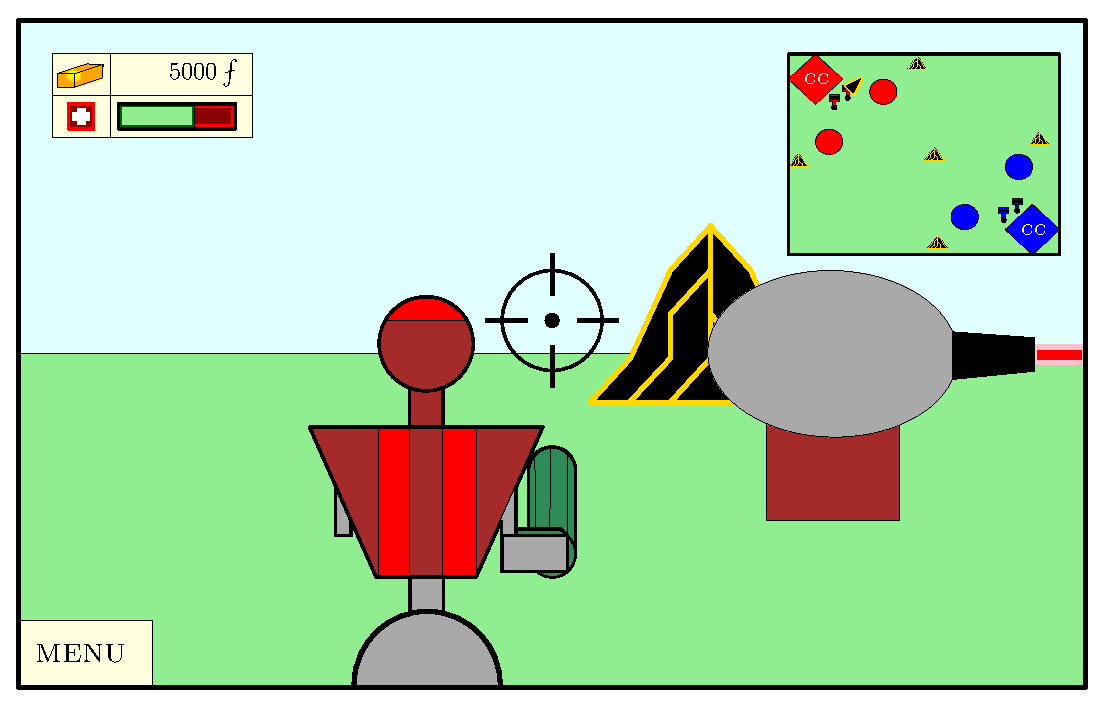
\includegraphics[width=0.9\textwidth]{Graphics/UI.eps}
    \caption{De gebruikersomgeving tijdens het spel}
    \label{fig:UI}
    \end{figure}
    De besturing van de robot kan met de \textsc{wasd}-toetsencombinatie of door gebruik te maken van de pijltjes-toetsen. Hiervoor geven we de volgende tabel:
    \begin{table}[H]
        \small
        \centering
        \begin{tabular}{| l | l |}
        \hline
        Knop & Reactie \\ \hline
        \textsc{w} of $\uparrow$ & De robot beweegt, indien mogelijk, vooruit naar de huidige kijkrichting toe \\ \hline
        \textsc{a} of $\leftarrow$ & De robot draait naar links \\ \hline
        \textsc{s} of $\downarrow$ & De robot beweegt, indien mogelijk, achteruit van de huidige kijkrichting af \\ \hline
        \textsc{d} of $\rightarrow$ & De robot draait naar rechts \\ \hline
        \end{tabular}
        \caption{Knoppen met bijbehorende reactie}
        \label{tab:planning}
    \end{table}

    De speler kan schieten door op de muis te drukken. Door de muis naar boven of naar beneden te bewegen, kijkt de speler verder omhoog of omlaag respectievelijk. Op analoge wijze kan de speler naar links of naar rechts draaien door respectievelijk de muis naar links of naar rechts te bewegen. Merk op dat het vizier altijd in het midden van het scherm blijft. De speler ziet dit dus doordat de horizon omlaag of omhoog schuift.
    \FloatBarrier
    \subsubsection{Schieten met het lasergeweer}
    Men kan opmerken uit figuur \ref{fig:UI} dat de schietrichting niet meteen duidelijk uit de gebruikersomgeving wordt. Immers, het vizier wordt niet op hetzelfde punt als het wapen op het scherm afgebeeld. Aangezien het vizier eenvoudiger is om mee te richten dan het wapen, wordt bij het schieten een laserstraal afgevuurd vanuit het wapen naar het punt waar het vizier op gericht staat. Dit is te zien in figuur \ref{fig:COL}. Als het vizier niet op een object gericht staat, dan zal, bij het schieten, de laserstraal uit het wapen afgevuurd worden in de kijkrichting.

    \begin{figure}[H]
    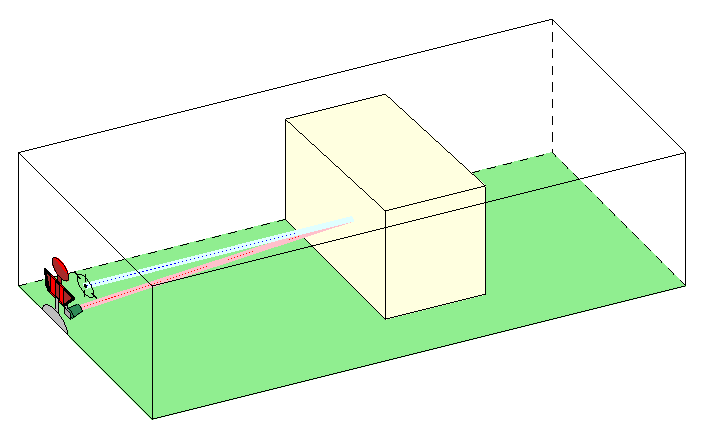
\includegraphics[width=0.9\textwidth]{Graphics/Collision.eps}
    \caption{Een voorbeeld van het schieten van het wapen, de blauwe lijn is niet zichtbaar tijdens het spelen}
    \label{fig:COL}
    \end{figure}

    Een probleem ontstaat wanneer er een object de laserstraal vanaf het wapen naar het punt, waar het vizier op gericht staat, blokkeert. Het object zou dan geraakt moeten worden en niet het punt waar het vizier op gericht staat. Er zijn twee manieren om dit op te lossen, men kan zeggen dat de laser altijd het punt van de vizier raakt. Dit is makkelijker te implementeren, aangezien we maar \'e\'en keer hoeven te bepalen waar een lijn een object raakt. Dit is te zien in figuur \ref{fig:COL2}. Een andere oplossing is dat in dit geval de laser alleen het object, dat in de weg staat, raakt. Dit is natuurlijk realistischer, maar minder makkelijk te implementeren. Dit is te zien in figuur \ref{fig:COL3}. In eerste instantie kiezen wij voor de eerste methode. Echter, indien de tijd ons de mogelijkheid gunt om de tweede oplossing te kunnen implementeren, zullen wij de tweede oplossing implementeren.
    \FloatBarrier
    \begin{figure}[h]
    \begin{subfigure}{0.45\textwidth}
    \centering
    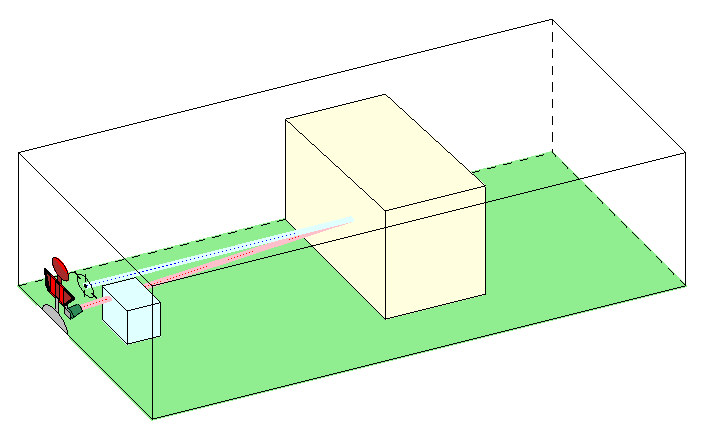
\includegraphics[width=\textwidth]{Graphics/Collision2.eps}
    \caption{De laser komt altijd aan op het punt aangewezen door het vizier}
    \label{fig:COL2}
    \end{subfigure}
    \begin{subfigure}{0.45\textwidth}
    \centering
    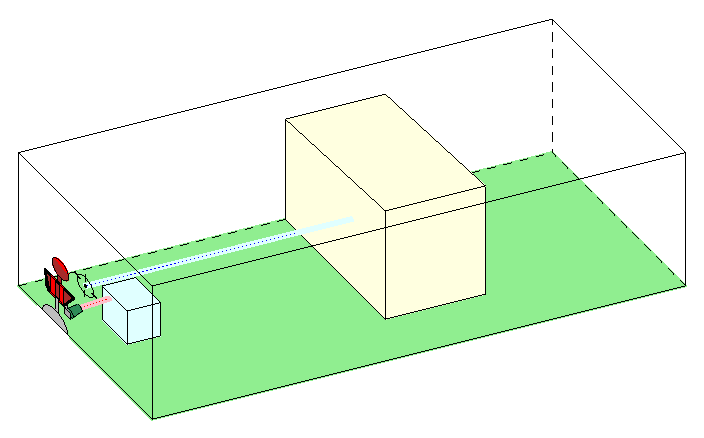
\includegraphics[width=\textwidth]{Graphics/Collision3.eps}
    \caption{De laser stopt zodra hij een ander object raakt}
    \label{fig:COL3}
    \end{subfigure}
    \caption{Oplossingen voor de problemen bij het schieten}
    \end{figure}

    \FloatBarrier
    \subsubsection{Het neerzetten van gebouwen}
    De speler kan ook opdracht geven om op een bepaalde plek een gebouw neer te laten zetten. Om een gebouw neer te zetten moet de speler eerst op de knop \textsc{b} drukken. Dan gaat de speler in de zogenaamde \emph{bouw-modus}. Op dat moment wordt er een klein menu onderaan het scherm van de speler afgebeeld. Door middel van sneltoetsen kan de speler een gebouw van dit menu kiezen.

    Merk op dat de muis op dit moment nog steeds de kijkrichting bestuurt. Als het gebouw gekozen is, wordt op de ondergrond een rooster getekend. Door middel van het vizier kan de speler een plek op het rooster aanwijzen. De speler kan door te klikken dan de opdracht geven om het gebouw neer te laten zetten. Op dat moment wordt de bijbehorende hoeveelheid goud uit de gezamenlijke kas gehaald. Vervolgens zal het gebouw ook worden neergezet.

    Als de speler niet genoeg goud in de gezamenlijke kas heeft voor het gebouw, wordt de speler gewaarschuwd. Dan wordt er natuurlijk geen goud uit de gezamenlijke kas gehaald en het gebouw niet neergezet. Na het neerzetten van het gebouw gaat de speler weer uit de bouw-modus. Op elk moment kan dit proces afgebroken worden door op de knop \textsc{b} te drukken. Dit kan gezien worden in figuur \ref{fig:gebouw}.

    \begin{figure}
    \centering
    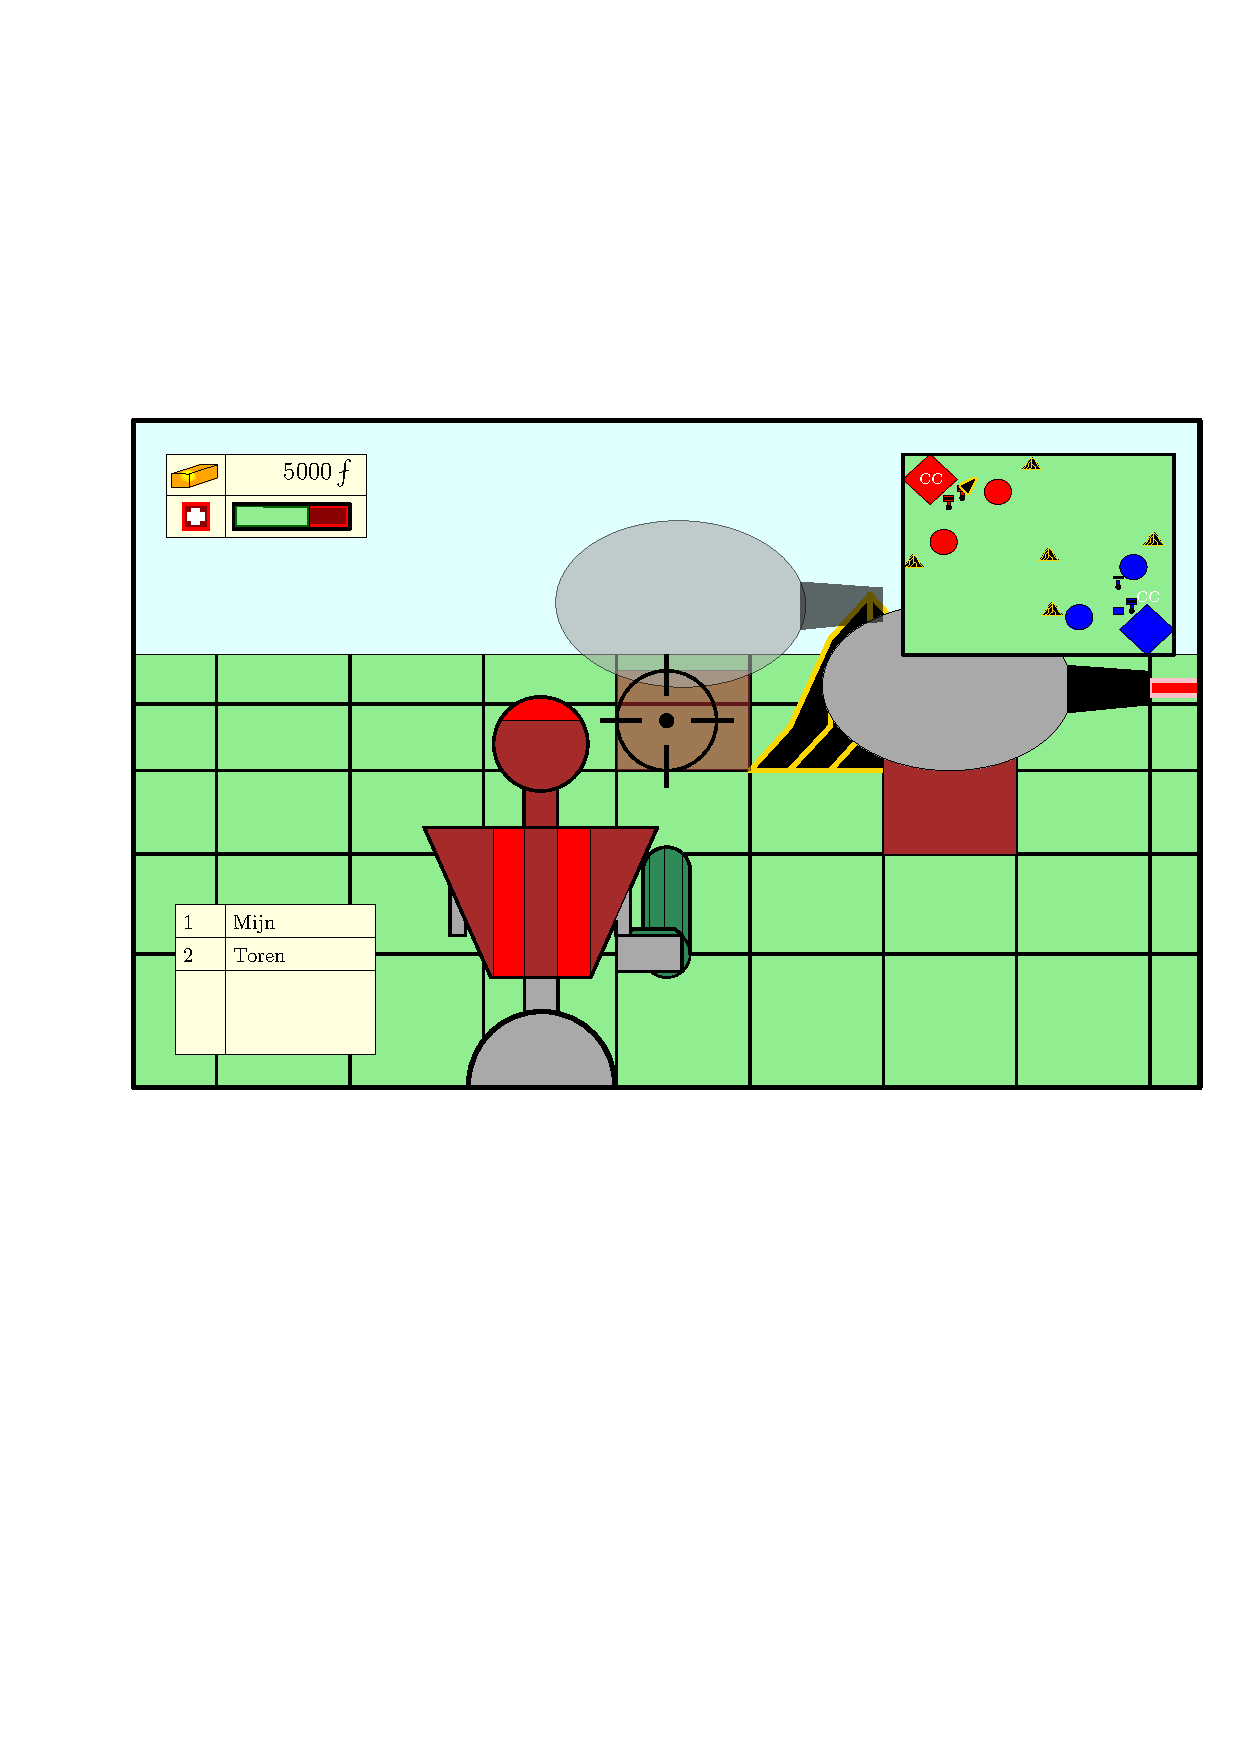
\includegraphics[width=\textwidth]{Graphics/UI2.pdf}
    \caption{Een voorbeeld van het neerzetten van een gebouw in de gebruikersomgeving}
    \label{fig:gebouw}
    \end{figure}

    \subsubsection{Optioneel}
    \label{sec:OPT}
    We hebben ook een aantal plannen voor uitbreiding van het spel. De volgende idee\"en zouden wij graag extra implementeren. De idee\"en zijn gesorteerd op aflopende volgorde van belangrijkheid.

    \begin{itemize}
    \item Extra goud, de gezamenlijke kas wordt periodiek met een vaste hoeveelheid verhoogd. Dit is dan additief met eventuele mijnen. Wij verwachten dat dit weinig tijd kost.
    \item Oorlogsmist, de robots hebben een beperkt zichtveld. Dit voorkomt dat spelers vanaf hun commandocentrum alle activiteiten van de tegenstanders kunnen zien. Wij denken dat dit weinig tijd kost.
    \item Plattegrond, zodat spelers een globaal overzicht krijgen van wat er op de kaart gebeurt. Dit kan eventueel ook weer met een oorlogsmist zijn, zodat de spelers alleen een gedeelte van het plattegrond kunnen zien, waar teamgenoten in de buurt staan. Wij vermoeden dat dit niet veel tijd kost.
    \item Muren, als een extra type gebouw. Onze bedoeling hierbij is dat deze muren relatief goedkoop zijn om te bouwen. Dit geeft een team meer opties om hun commandocentrum of delfplaatsen te beschermen. Bovendien geeft het de extra mogelijkheid om een veilige plek te cre\"eren, waarvandaan tegenstanders aangevallen kunnen worden. Wij voorzien dat dit een kleine hoeveelheid tijd kost.
    \item Ontwikkelingen, de spelers krijgen ontwikkelingspunten tijdens het spel. Deze kunnen worden verdiend door het uitschakelen van spelers, werkers, infanterie en het vernietigen van gebouwen. Werkers en infanterie worden uitgelegd in de volgende twee idee\"en. Hiermee kunnen de spelers bijvoorbeeld de eigenschappen van hun robot verbeteren, zoals de snelheid van lopen en hoe sterk het harnas is. Ook is het mogelijk om sterkere wapens te kopen. Wij denken dat dit veel tijd kost, aangezien een `winkel' gemaakt moet worden waar deze punten gespendeerd kunnen worden. Ook moeten de eigenschappen van een speler dynamisch gemaakt worden.
    \item Werkers, dit zijn computergestuurde robots. Zodra een speler daartoe opdracht geeft, komen werkers uit het commandocentrum van het bijbehorende team om een gebouw neer te zetten. Dit vervangt de oude mogelijkheid van spelers om te bouwen. Een gevolg van deze aanpassing is dat het langer duurt om een gebouw te bouwen als de afstand van de bouwplaats tot het commandocentrum groter is. Bovendien wordt het mogelijk om het bouwen van het andere team te vertragen door de werkers uit te schakelen. Dit kost heel veel tijd, aangezien de werkers gedistribueerd bestuurd worden. Hiervoor is dus een soort gedistribueerde kunstmatige intelligentie nodig. Dit is een uitdaging. Merk ook op, dat deze computergestuurde robots niet door de gebouwen horen te lopen, waardoor deze kunstmatige intelligentie totaal niet triviaal is.
    \item Infanterie, ook dit zijn computergestuurde robots. Deze kunnen door spelers worden gekocht, vanaf het commandocentrum lopen ze naar gebouwen van het andere team om deze gebouwen aan te vallen. Dit kost nog meer tijd dan de werkers, aangezien de infanterie niet tussen twee vaste punten zich moeten verplaatsen, maar ook gebouwen moeten kunnen aanvallen.
    \end{itemize} 

    \subsection{Het ontwerp}
    % Inclusief alternatieven, motivering van keuzes, aannames en communicatieprotocol

    \subsection{Conclusie}
    % Met daarin reflectie over het verloop van het project en het groepsproces daarbij

    \section{Evaluatie}
    % Wat is bereikt
    % Hoe het project is verlopen

    \section{Literatuurlijst}

    \newpage
    \appendix
    \section{Begrippenlijst}
    % Andere appendices

\end{document} 